\section{字体排印}

\begin{frame}{先看一个例子}
\begin{minipage}{\textwidth}
  \SimHei\small
  \hyphenpenalty=10000\hbadness=10000\linespread{0.8}\selectfont
  \textbf{Typography} is the art and technique of arranging type to make written language
  legible,readable,and appealing when displayed. The arrangement of type involves selecting
  typefaces, point sizes, line lengths, line-spacing(\textit{leading}), and letter-spacing
  (\textit{tracking}), and adjusting the space between pairs of letters(\textit{kerning}).
  The term typography is also applied to the style,arrangement, and appearance of the letters,
  numbers, and symbols created by the process. \textbf{Type design} is a closely related craft,
  sometimes considered part of typography;most typographers do not design typefaces, and some
  type designers do not consider themselves typographers. Typography also may be used as a
  decorative device,unrelated to communication of information.
\end{minipage}
\nonumberfootnote{中易黑体,行距 0.8 倍,关闭断词;来源:
  \link{https://en.wikipedia.org/wiki/Typography}}
\end{frame}

\begin{frame}{没有对比就没有伤害}
\begin{minipage}{\textwidth}
  \EBGaramond\small
  \textbf{Typography} is the art and technique of arranging type to make written language
  legible, readable, and appealing when displayed. The arrangement of type involves selecting
  typefaces, point sizes, line lengths, line-spacing (\textit{leading}), and letter-spacing
  (\textit{tracking}), and adjusting the space between pairs of letters (\textit{kerning}).
  The term typography is also applied to the style, arrangement, and appearance of the letters,
  numbers, and symbols created by the process. \textbf{Type design} is a closely related craft,
  sometimes considered part of typography; most typographers do not design typefaces, and some
  type designers do not consider themselves typographers. Typography also may be used as a
  decorative device, unrelated to communication of information.
\end{minipage}
\nonumberfootnote{EB Garamond,默认设置}
\end{frame}

\begin{frame}{术语}
\footnotesize
\begin{columns}[t]
\begin{column}{0.48\textwidth}
  \begin{itemize}
    \item 语言\zhparen{language}
    \item 文字\zhparen{script}
    \item 书写系统\zhparen{writting system}
    %
    \item 符号\zhparen{symbol}
    \item 字符\zhparen{character}
    \item 字符形\zhparen{glyph}
    %
    \item 字符集\zhparen{character set}
    \item 编码\zhparen{encoding}
    \item 码位\zhparen{code point}
  \end{itemize}
\end{column}
\begin{column}{0.48\textwidth}
  \begin{itemize}
    \item 字体\zhparen{font}
    \item 字型\zhparen{typeface}
    %
    \item 易认性\zhparen{legibility}
    \item 可读性\zhparen{readability}
    %
    \item 字偶间距\zhparen{kerning}
    \item 字距\zhparen{tracking}
    %
    \item 栅格化\zhparen{rasterization}
    \item 渲染提示\zhparen{hinting}
    \item ……
  \end{itemize}
\end{column}
\end{columns}
\end{frame}

\begin{frame}[standout]
  \large \textbf{\LaTeX{} will do (almost) all the things for you.}
\end{frame}

\begin{frame}[fragile]
\frametitle{Punctuations: hyphen/dash}
\begin{columns}
\begin{column}{0.84\textwidth}
  \begin{itemize}
    \item<1-> Hyphen \enparen{\usv{002D}}: |-|

      \begin{itemize}
        \item Four-dimensional momentum
        \item Hyphenation
      \end{itemize}

    \item<3-> En dash \enparen{\usv{2013}}: |--|

      \begin{itemize}
        \item Ryu--Takayanagi formula (\emph{cf.} Levi-Civita symbol)
        \item pp.~187--189
      \end{itemize}

    \item<4-> Em dash \enparen{\usv{2014}}: |---|

      \begin{itemize}
        \item Red, white, and blue---these are the colors of the flag
        \item Like colon, parentheses, \emph{etc.}
      \end{itemize}

    \item<5-> Minus \enparen{\usv{2212}}: |$-$|

      \begin{itemize}
        \item $a-b$, $-a$
      \end{itemize}
  \end{itemize}
\end{column}
\begin{column}{0.13\textwidth}
  \onslide<2->
  \tiny\RaggedRight
  A hyphen\alert{-}ation algo\alert{-}rithm is a set of rules, especially one codified
  for imple\alert{-}mentation in a computer program, that decides at which points
  a word can be broken over two lines with a hyphen.
\end{column}
\end{columns}
\end{frame}

\begin{frame}[fragile]
\frametitle{Punctuations: quotation mark}
\begin{itemize}
  \item<1-> Left/right, single/double:

    \begin{itemize}
      \item `\ldots{}' \enparen{\usv{2018}, \usv{2019}}: |`...'|
      \item ``\ldots{}'' \enparen{\usv{201C}, \usv{201D}}: |``...''|
    \end{itemize}

  \item<2-> Different languages:

    \begin{itemize}
      \item `British ``English'' style' and ``American `English' style''
      \item „German'', ''Finnish'', «French», »Danish«, \emph{etc.}
      \item<3-> Use \pkg{csquotes} package
    \end{itemize}

  \item<4-> Programming:

    \begin{itemize}
      \item |char* my_name = "Xiangdong Zeng";|
    \end{itemize}

  \item<5-> Mathematics:

    \begin{itemize}
      \item |f'| = |f^{\prime}|: $f'(x) = f^{\prime}(x)$
    \end{itemize}
\end{itemize}
\end{frame}

\begin{frame}[fragile]
\frametitle{中文标点符号}
\begin{itemize}
  \item<+-> 句号

    \begin{itemize}
      \item 正常文本。科技文本.
    \end{itemize}

  \item<+-> 引号

    \begin{itemize}
      \item 『传统风格』,「某乎风格」,“标准风格”,\mbox{}’\kern-0.6em奇葩风格”
    \end{itemize}

  \item<+-> 破折号

    \begin{itemize}
      \item 断开{\SourceHanSerif\symbol{"2014}\symbol{"2014}}是不好的,
            不断开——是好的
    \end{itemize}

  \item<+-> 波浪号:

    \begin{itemize}
      \item |~| ≠ |\textasciitilde| ≠ |\texttildelow| ≠ |$\sim$| ≠ 你要的那一个
      \item 那就是~青\textasciitilde 藏\texttildelow 高 $\sim$ 原~~~~

        \begin{itemize}
          \item \texttt{\usv{007E}: Tilde}
          \item \texttt{\usv{02F7}: Modifier letter low tilde}
          \item \texttt{\usv{223C}: Tilde operator}
          \item \texttt{\usv{FF5E}: Fullwidth tilde}
          \item \ldots{}
        \end{itemize}
    \end{itemize}
\end{itemize}
\end{frame}

\begin{frame}{大家来找茬 \texorpdfstring{\EmojiOne 😎}{😎}}
\begin{center}
  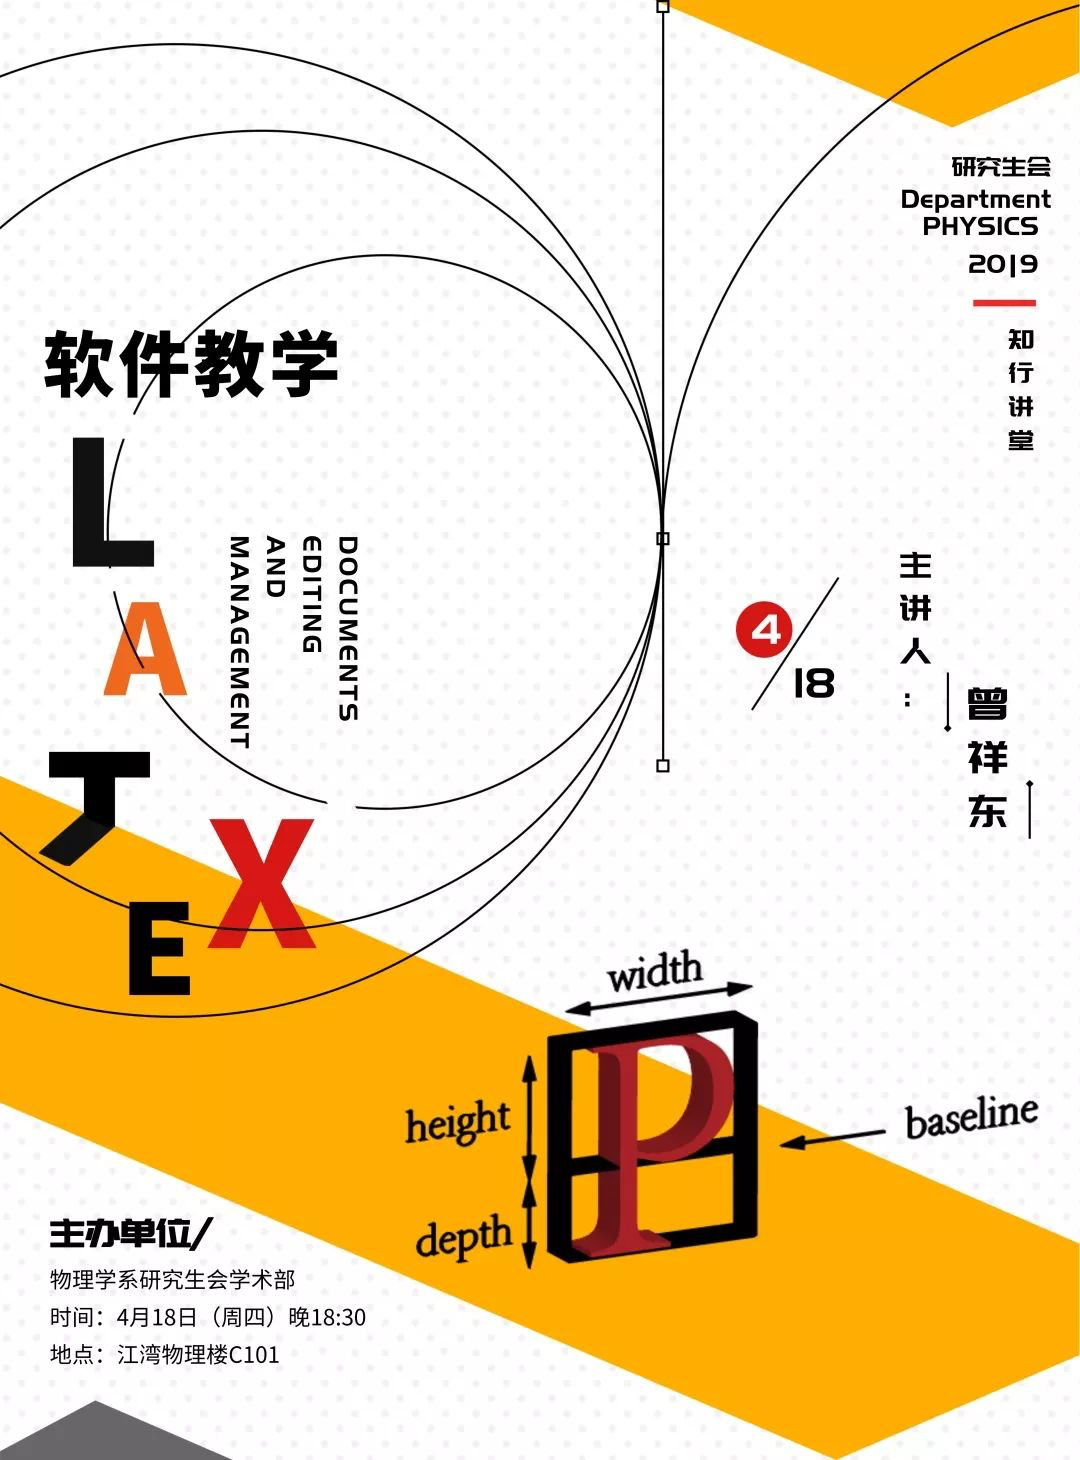
\includegraphics[width=5.6cm]{figures/poster-hd.png}
\end{center}
\vspace{-0.5cm}
\end{frame}

\begin{frame}{使用字体:\pkg{fontspec} 宏包}
\begin{itemize}
  \item<1-> 字体家族

    \begin{itemize}
      \item 衬线体:
        {\EBGaramond EB Garamond},
        {\TimesNewRoman Times New Roman},
        {\LatinRomanX Latin Modern}, \emph{etc.}
      \item 无衬线体:
        {\Helvetica Helvetica Neue},
        {\Avenir Avenir Next},
        {\Optima Optima}, \emph{etc.}
      \item 等宽字体:
        {\Courier Courier},
        {\Menlo Menlo},
        \texttt{Iosevka}, \emph{etc.}
      \item 中文字体:宋体、{\HeiTi 黑体}、{\FangSong 仿宋}、{\KaiTi 楷书}、{\WaWa (娃娃体)}……
    \end{itemize}

  \item<2-> 样式

    \begin{itemize}
      \item 粗体、意大利体:
        \textbf{Bold} vs {\addfontfeatures{AutoFakeBold=4}\textbf{Faked bold}},
        \textit{Italic} vs {\addfontfeatures{AutoFakeSlant=0.2}\textsl{Slant}}
      \item<3-> \alert{汉字一般不使用斜体}
      \item<4-> 视觉字号\zhparen{optical size}:\\
        {\LatinRomanV    Tiny},
        {\LatinRomanVI   Script},
        {\LatinRomanVII  Footnote},
        {\LatinRomanVIII Caption},
        {\LatinRomanIX   Small},
        {\LatinRomanX    Normal},
        {\LatinRomanXII  Large},
        {\LatinRomanXVII Huge}
    \end{itemize}

  \item<5-> OpenType 特性

    \begin{itemize}
      \item 连字\zhparen{ligature}:{f}{f} $\to$ ff, {f}{i} $\to$ fi, {f}{l} $\to$ fl
      \item 老式数字\zhparen{old-style number}:
        0123456789 $\to$ {\addfontfeatures{Numbers=OldStyle}0123456789}
      \item 字偶间距\zhparen{kerning}:{T}{y} $\to$ Ty, {W}{A} $\to$ WA
    \end{itemize}

  \item<6-> \alert{请避免滥用过多字体{\tiny (此页除外)}}
\end{itemize}
\vspace{-0.2cm}
\end{frame}
